\chapter{Gráficas del Análisis Exploratorio de datos}
\begin{subappendices}

\section{Definición de Variables}
	\label{appendix:A}
\begin{table}[!ht]
	\caption{Nomenclatura de las Variables}
	\centering
	\resizebox{\linewidth}{!}{	\begin{tabular}{|c|c|c|}
			\hline 
			\textbf{	Nombre de la variable} & \textbf{Significado} & \textbf{Valores} \\ 
			\hline 
			CDGENERICO & Indica el código genérico del centro & 
			\begin{minipage}[t]{0.4\textwidth}
				\begin{itemize}
					\item CIMELPR PRSEC = 16
					\item CIMPR SEC = 17
					\item CEPA = 31
					\item CREI = 39
					\item IES = 42
					\item CPR ES = 45
					\item SIES = 47
					\item CPR FPE = 58
					\item CP IFP = 68
					\item CP INF-PRI-SEC = 70
					\item CPR INF-PRI-SEC = 72
					\item CPR PRI-SEC = 73 
				\end{itemize}
			\end{minipage}  \\ 
			\hline 
			CDNATURALEZA & Indica la naturaleza del centro. Centros públicos y privados & 
			\begin{minipage}[t]{0.4\textwidth}
				\begin{itemize}
					\item Público = 1
					\item Privado = 2
				\end{itemize}
			\end{minipage} \\ 
			\hline 
			CDPOSTAL & Código postal del centro &  \\ 
			\hline 
			ITCOMEDOR & Disponibilidad de comedor en el centro &  		\begin{minipage}[t]{0.4\textwidth}
				\begin{itemize}
					\item No = 1
					\item Si = 2
				\end{itemize}
			\end{minipage}\\ 
			\hline 
			ITTRANSPORTE & Disponibilidad de transporte & \begin{minipage}[t]{0.4\textwidth}
				\begin{itemize}
					\item No = 1
					\item Si = 2
				\end{itemize}
			\end{minipage}\\ 
			\hline 
			ITBILINGUE & Disponibilidad de bilingüismo & \begin{minipage}[t]{0.4\textwidth}
				\begin{itemize}
					\item No = 1
					\item Si = 2
				\end{itemize}
			\end{minipage}\\ 
			\hline 
			CD\_NIVEL & Nivel educativo del grupo &    
			\begin{minipage}[t]{0.4\textwidth}
				\begin{itemize}
					\item Bachillerato = 5
					\item Educación Secundaria Obligatoria = 13
					\item Módulos Profesionales = 14
					\item Formación Profesional GM = 15
					\item Formación Profesional GS = 16
				\end{itemize}
			\end{minipage}\\ 
			\hline 
			NM\_CURSO & Curso del nivel educativo del grupo &  
			\begin{minipage}[t]{0.4\textwidth}
				\begin{itemize}
					\item Primero = 1
					\item Segundo = 2
					\item Tercero = 3
					\item Cuarto = 4
				\end{itemize}
			\end{minipage}\\ 
			\hline 
			NM\_UNIDADES & Número de grupos para un determinado nivel y un numero de curso &  \\ 
			\hline 
			NM\_ALUMNOS & Número de alumnos para un determinado nivel y numero de curso &  \\ 
			\hline 
			RATIO & Ratio de alumnos por grupo para cada nivel y numero de curso. &  \\ 
			\hline 
			GRUPO\_PREDECIR & Grupo a predecir  &  \\ 
			\hline 
	\end{tabular}}
	
	\label{tab:TablaVariables}
\end{table}

\section{Análisis exploratorio}
\subsection{Estadísticos mas relevantes}
\begin{figure*}[htb]
	\centering
	\caption{Estadisticos de las variables. Elaboración propia}
	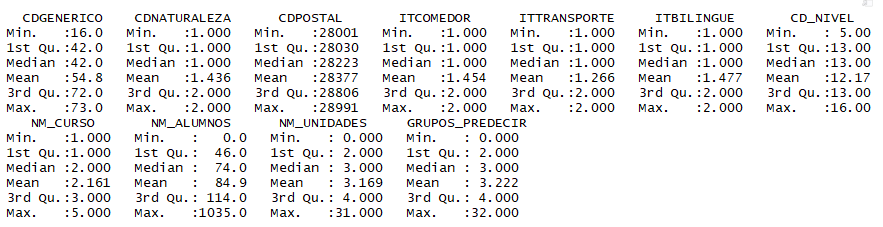
\includegraphics[width=1\textwidth]{recursos/ImagenesR/estadisticos}
	\label{fig:estadisticos}
\end{figure*}
\FloatBarrier

\begin{figure*}[htb]
	\centering
	\caption{Diagrama de cajas normalizado. Elaboración propia}
	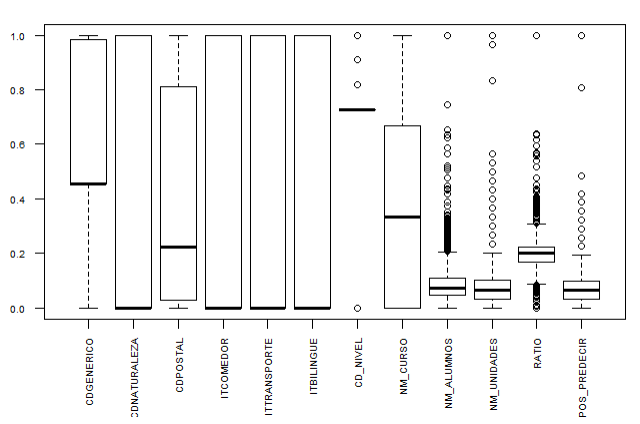
\includegraphics[width=0.8\textwidth]{recursos/ImagenesR/boxplotNorm}
	\label{fig:boxplotNorm}
\end{figure*}
\FloatBarrier

Como se puede observar en la figura \ref{fig:boxplotNorm}, las variables de NMALUMNOS, NMUNIDADES y RATIO contienen datos anómalos. En el caso de la variable NM\_ALUMNOS, existen centros que tienen números demasiado elevados de alumnos para un determinado nivel educativo, esto se debe a que dichos centros tienen la modalidad de distancia para esos niveles educativos. Relacionado con el caso anterior es el NM\_UNIDADES que, al igual que los alumnos, se dispara a números elevados. Se debe de la misma forma a la modalidad de distancia.

\subsection{Análisis de normalidad}
En primer lugar, se pueden ver la densidad de las variables individualmente de observar a simple vista si cumplen o no con una distribución normal.

\begin{figure*}[htb]
	\centering
	\caption{Distribución 1. Elaboración propia}
	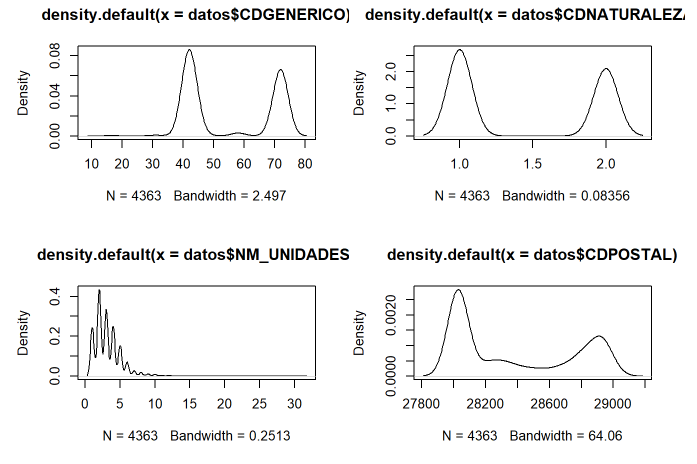
\includegraphics[width=0.8\textwidth]{recursos/ImagenesR/norm1}
	\label{fig:norm1}
\end{figure*}
\FloatBarrier

\begin{figure*}[htb]
	\centering
	\caption{Distribución 2. Elaboración propia}
	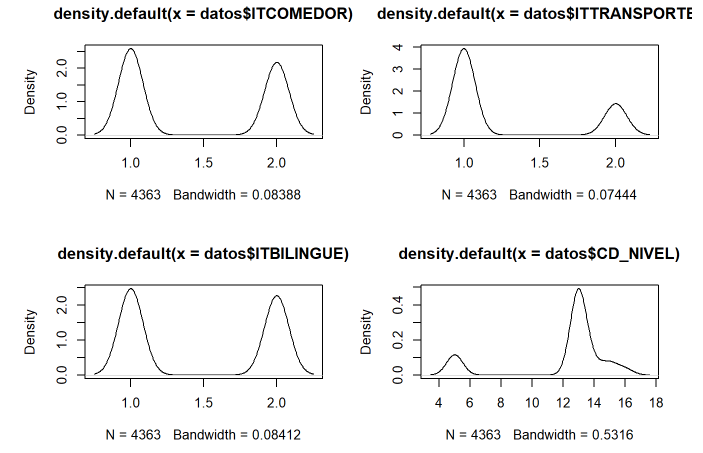
\includegraphics[width=0.8\textwidth]{recursos/ImagenesR/norm2}
	\label{fig:norm2}
\end{figure*}
\FloatBarrier

\begin{figure*}[htb]
	\centering
	\caption{Distribución 3. Elaboración propia}
	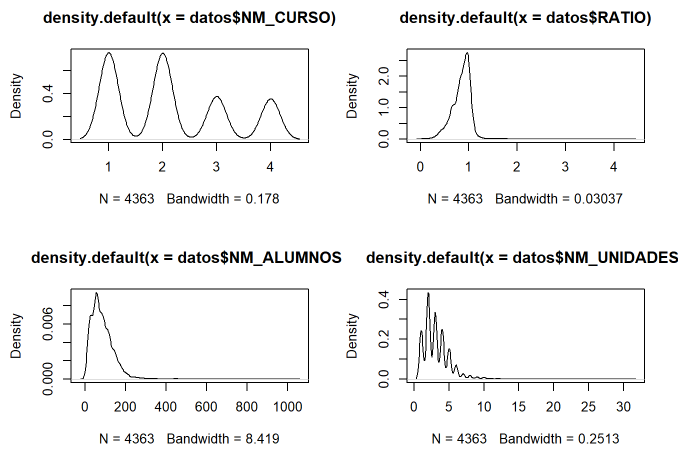
\includegraphics[width=0.8\textwidth]{recursos/ImagenesR/norm3}
	\label{fig:norm3}
\end{figure*}
\FloatBarrier

\begin{figure*}[htb]
	\centering
	\caption{Diagrama de barras 1. Elaboración propia}
	\includegraphics[width=0.8\textwidth]{recursos/ImagenesR/barplot1}
	\label{fig:barplot1}
\end{figure*}
\FloatBarrier

\begin{figure*}[htb]
	\centering
	\caption{Diagrama de barras 2. Elaboración propia}
	\includegraphics[width=0.8\textwidth]{recursos/ImagenesR/barplot2}
	\label{fig:barplot2}
\end{figure*}
\FloatBarrier

Tanto en la figuras \ref{fig:barplot1} y \ref{fig:barplot2} se puede hacer una comparativa sobre los servicios que ofrecen los centros. Se puede observar como la mayoria de centros no tienen transporte. Existe un ligero numero de centros que tiene comedor sobre centros que no tienen, de la misma manera ocurre con el bilingüismo. La mayoría de los datos que se tiene son del nivel 13, que corresponde con la Educación Secundaria Obligatoria y la mayoría de estos datos corresponden a centros con el codigo generico 42 y 72 (IES y CPR INF-PRI-SEC, respectivamente).

\subsection{Relaciones entre variables}
Para el estudio de la correlación se utiliza el Coeficiente de Correlación de Pearson (R).
\begin{figure*}[htb]
	\centering
	\caption{Matriz de correlaciones. Elaboración propia}
	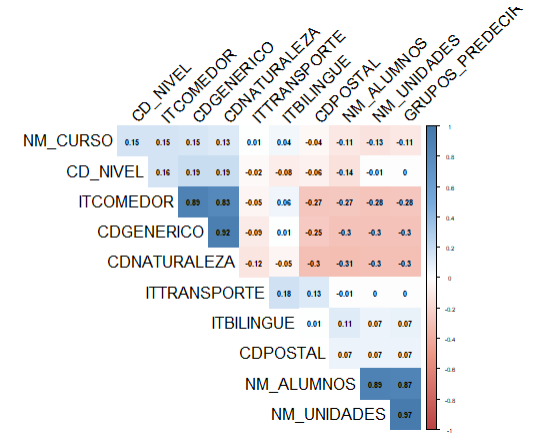
\includegraphics[width=0.8\textwidth]{recursos/ImagenesR/matrizcorrelacion}
	\label{fig:matrizcorrelaciones}
\end{figure*}
\FloatBarrier


\begin{figure*}[htb]
	\centering
	\caption{Variables más correladas. Elaboración propia}
	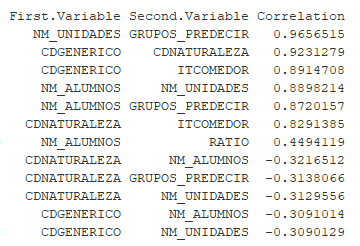
\includegraphics[width=0.6\textwidth]{recursos/ImagenesR/mayorescorrelaciones}
	\label{fig:mayorescorrelaciones}
\end{figure*}
\FloatBarrier

\begin{figure*}[htb]
	\centering
	\caption{Mayor correlación con variable a predecir. Elaboración propia}
	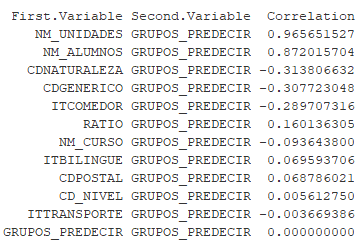
\includegraphics[width=0.6\textwidth]{recursos/ImagenesR/mayorcorrelacion}
	\label{fig:mayorcorrelacionpredecir}
\end{figure*}
\FloatBarrier
En las figuras \ref{fig:matrizcorrelaciones}, \ref{fig:mayorescorrelaciones} y \ref{fig:mayorcorrelacionpredecir} se muestra prácticamente la misma información, la correlación entre variables. En la figura \ref{fig:mayorescorrelaciones} se muestran aquellos pares de variables que poseen la mayor correlación. Se puede apreciar en esta figura que la variable NMUNIDADES y GRUPOSPREDECIR tienen una correlación casi perfecta, lo que implica que aportarían la misma información al conjunto de datos.

En la figura \ref{fig:mayorcorrelacionpredecir} se muestran aquellas variables que tienen mayor correlación con la variable a predecir. Podemos observar que las variables de NMUNIDADES y NMALUMNOS tienen una enorme correlación con la variable a predecir. Esta relación es lógica, ya que a mayor numero de alumnos o grupos, la variable a predecir aumenta. También se puede destacar que la naturaleza (publica o privada) de un centro esta relacionada con el numero de grupos a predecir. Al aumentar el valor de la naturaleza, disminuye el numero de unidades. De esta premisa se puede deducir que los padres suelen matricular a sus hijos en centros públicos, y por lo tanto, el numero de grupos tiende a aumentar. El servicio de comedor también es un factor con relación con el numero de grupos, lo que implica que los padres suelen matricular a los alumnos en centros que dispongan del servicio de comedor.

\begin{figure*}[htb]
	\centering
	\caption{Correlación entre variables NM\_ALUMNOS y NM\_GRUPOS. Elaboración propia}
	\label{fig:relacionAlumnGrup}
	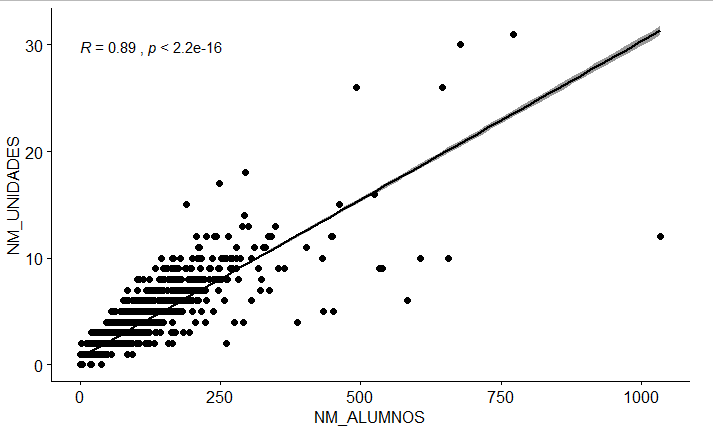
\includegraphics[width=0.6\textwidth]{recursos/ImagenesR/RelacionAlumnGrupos}
	
\end{figure*}
\FloatBarrier

\begin{figure*}[htb]
	\centering
	\caption{Correlación entre variables NM\_UNIDADES y GRUPOS\_PREDECIR. Elaboración propia}
	\label{fig:RelacionGruposYUnidades}
	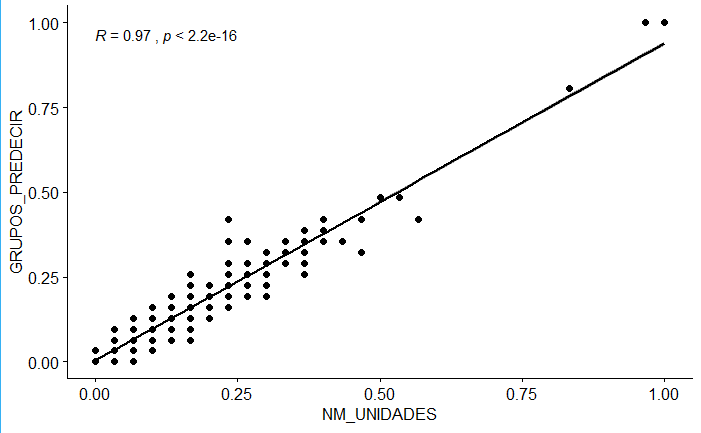
\includegraphics[width=0.6\textwidth]{recursos/ImagenesR/RelacionGruposYUnidades}
	
\end{figure*}
\FloatBarrier

\section{Selección de Variables}
\subsection{Usando Random Forest}
\begin{figure*}[htb]
	\centering
	\caption{Variables más importantes usando Random Forest. Elaboración propia}
	\label{fig:VarImpRF}
	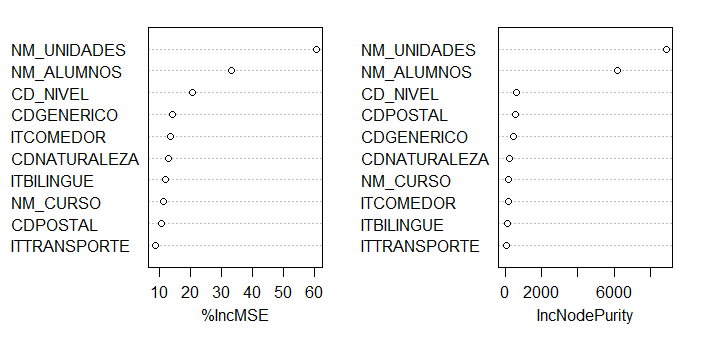
\includegraphics[width=0.6\textwidth]{recursos/ImagenesR/VarImpRF}
	
\end{figure*}
\FloatBarrier
La variable \textbf{IncNodePurity} se la conoce también como la media de decrecimiento de de Gini. El indice de Gini es una ``medida de desorden'' en este caso IncNodePurity tiene el siguiente sentido, a mayor medida, mayor importancia en los modelos creados, puesto que valores próximos a 0 implican un mayor desorden. Por tanto, si computamos la media del "decrecimiento" del indice de Gini cuanto mayor sea esta medida, mas variabilidad aporta a la variable dependiente.

Por otro lado, la variable \textbf{IncMSE} es la media de decrecimiento en la precisión, y es también un indicador sobre la importancia de las variables en el modelo.
\subsection{Regresión Paso a Paso}
La regresión por pasos (Stepwise Regression) consiste en añadir o eliminar iterativamente predicadores en el modelo predictivo, con el objetivo de encontrar el subconjunto de los datos que obtengan mayor precisión en el modelo o, dicho de otra forma, reducir el error en la predicción. \cite{kassambara2018}

Existen 3 estrategias para realizar la regresión paso a paso: backward, forward y stepwise.

\subsubsection{Usando Backward Selection}
\begin{figure*}[htb]
	\centering
	\caption{Resultado Backward Selection. Elaboración propia}
	\label{fig:backwardSum}
	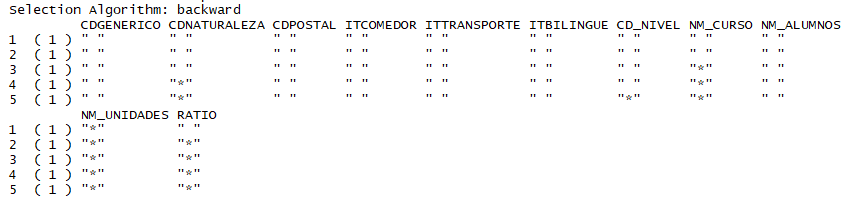
\includegraphics[width=1\textwidth]{recursos/ImagenesR/backwardSum}
	
\end{figure*}
\FloatBarrier

Los asteriscos en los resultados indican los predictores que se deben tomar para realizar el modelo. En este caso se necesitan las variables CD\_NATURALEZA, CD\_NIVEL, NM\_CURSO, NM\_UNIDADES y RATIO.

\begin{figure*}[htb]
	\centering
	\caption{Gráfico Backward Selection. Elaboración propia}
	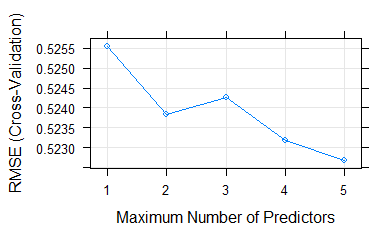
\includegraphics[width=0.6\textwidth]{recursos/ImagenesR/backward}
	\label{fig:backward}
\end{figure*}
\FloatBarrier

En la figura \ref{fig:backward} se puede observar como la mejor precision se obtiene utilizando los 5 predictores de la figura \ref{fig:backwardSum}.

\subsubsection{Usando Stepwise Selection}
\begin{figure*}[htb]
	\centering
	\caption{Resultado Stepwise Selection. Elaboración propia}
	\label{fig:seqSum}
	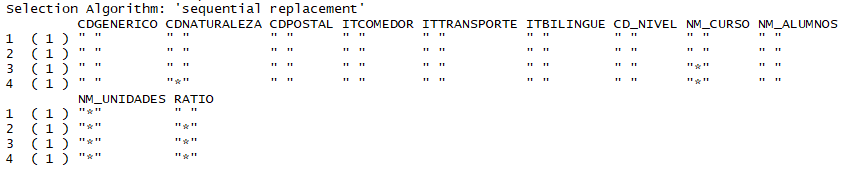
\includegraphics[width=1\textwidth]{recursos/ImagenesR/seqSum}
	
\end{figure*}
\FloatBarrier

Nuevamente los asteriscos de la figura \ref{fig:seqSum} indican aquellos predictores que deben utilizarse, en este caso son: CD\_NATURALEZA, NM\_CURSO, NM\_UNIDADES y RATIO.

\begin{figure*}[htb]
	\centering
	\caption{Gráfico Stepwise Selection. Elaboración propia}
	\label{fig:seq}
	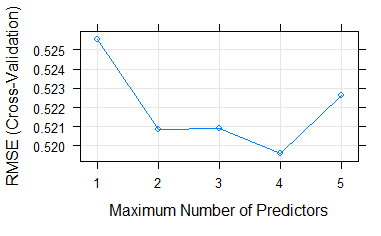
\includegraphics[width=0.6\textwidth]{recursos/ImagenesR/seq}
	
\end{figure*}
\FloatBarrier

En la figura \ref{fig:seq} se puede observar como la mayor precisión (menor valor de RMSE) se obtiene utilizando 4 variables.


\subsubsection{Usando Forward Selection}
\begin{figure*}[htb]
	\centering
	\caption{Resultado Forward Selection. Elaboración propia}
	\label{fig:fordwardSum}
	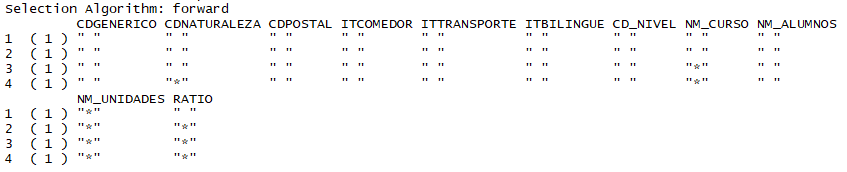
\includegraphics[width=1\textwidth]{recursos/ImagenesR/fordwardSum}
\end{figure*}
\FloatBarrier

En los resultados de la figura \ref{fig:fordwardSum} se puede observar como nuevamente se tienen en cuenta las variables CD\_NATURALEZA, NM\_CURSO, NM\_UNIDADES y RATIO.

\begin{figure*}[htb]
	\centering
	\caption{Gráfico Forward Selection. Elaboración propia}
	\label{fig:fordward}
	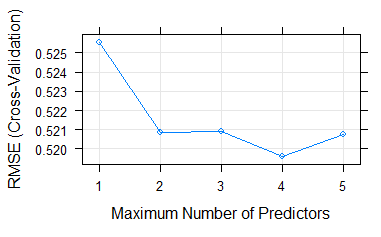
\includegraphics[width=0.6\textwidth]{recursos/ImagenesR/fordward}
\end{figure*}
\FloatBarrier

Al igual que en la estrategia de ``Stepwise'', se ha obtenido el mejor resultado de RMSE utilizando 4 variables. Estas variables son las obtenidas en el resultado de la figura \ref{fig:fordwardSum}.	
\end{subappendices}



\chapter{Análisis Predictivo}
\begin{subappendices}
	\label{appendix:A}
\section{Comparación de Modelos}

K-VECINOS CERCANOS
\begin{figure*}[htb]
	\centering
	\caption{K-Vecinos Cercanos. Elaboración propia}
		\label{fig:knnSUM}
	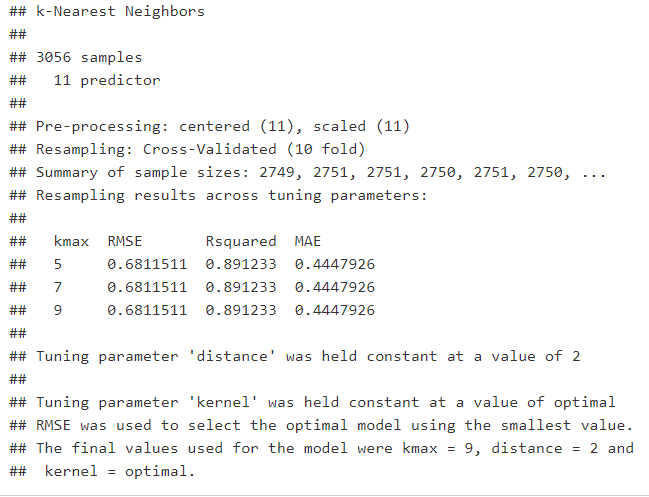
\includegraphics[width=0.6\textwidth]{recursos/ImagenesR/knnSUM}
\end{figure*}
\FloatBarrier
REDES NEURONALES
\begin{figure*}[htb]
	\centering
	\caption{Redes Neuronales. Elaboración propia}
		\label{fig:nnSUM}
	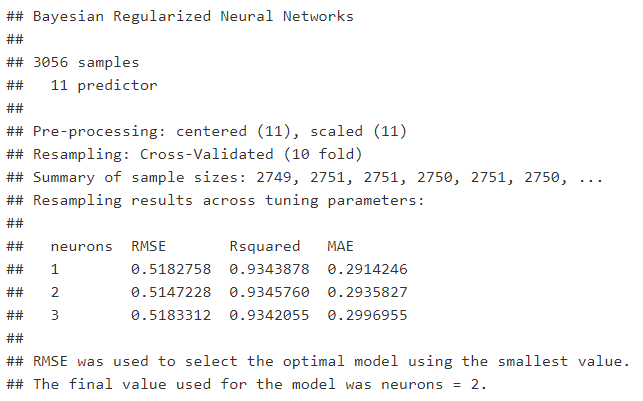
\includegraphics[width=0.6\textwidth]{recursos/ImagenesR/nnSUM}
\end{figure*}
\FloatBarrier

\begin{figure*}[htb]
	\centering
	\caption{Regresión Logística. Elaboración propia}
		\label{fig:regSUM}
	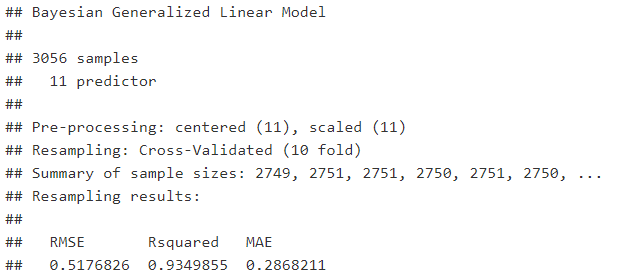
\includegraphics[width=0.6\textwidth]{recursos/ImagenesR/regSUM}
\end{figure*}
\FloatBarrier
SVM
\begin{figure*}[htb]
	\centering
	\caption{SVM. Elaboración propia}
		\label{fig:svmSUM}
	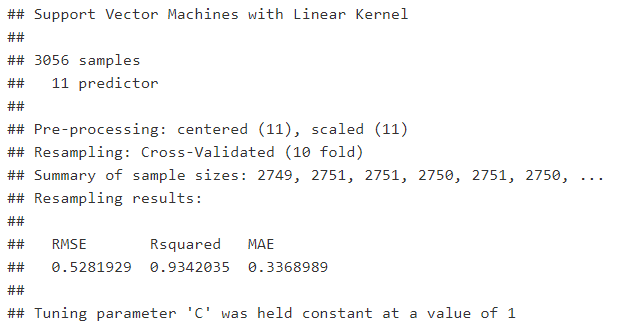
\includegraphics[width=0.6\textwidth]{recursos/ImagenesR/svmSUM}
\end{figure*}
\FloatBarrier

\begin{figure*}[htb]
	\centering
	\caption{Arbol de Decisión. Elaboración propia}
		\label{fig:treeSUM}
	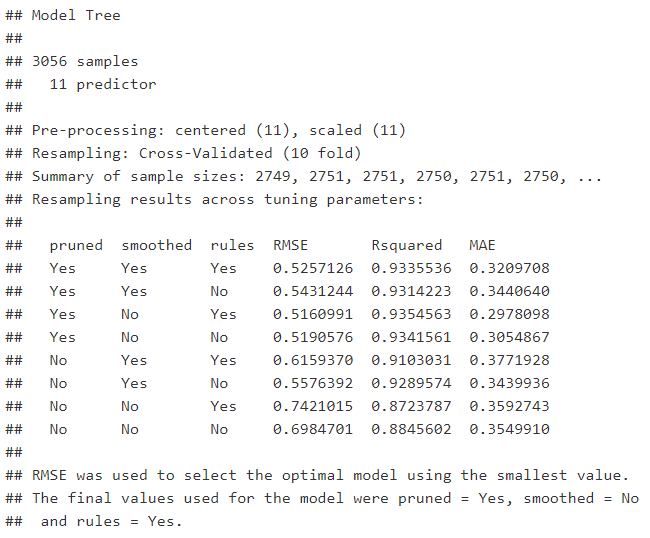
\includegraphics[width=0.6\textwidth]{recursos/ImagenesR/treeSUM}

\end{figure*}
\FloatBarrier

\begin{table}[!ht]
	\caption{Precisión de Modelos}
		\label{fig:ComparacionModelos}
\centering
\begin{tabular}{|c|c|c|c|c|c|}
	\hline 
	kknn & brnn & rf & svmLinear     & M5  & bayesglm \\ 
	\hline 
	0.681 & 0.515 & 0.576 & 0.528 & 0.516 & 0.518 \\ 
	\hline 
\end{tabular} 
\end{table}

\begin{figure*}[htb]
	\centering
	\caption{Comparación de Modelos. Elaboración propia}
	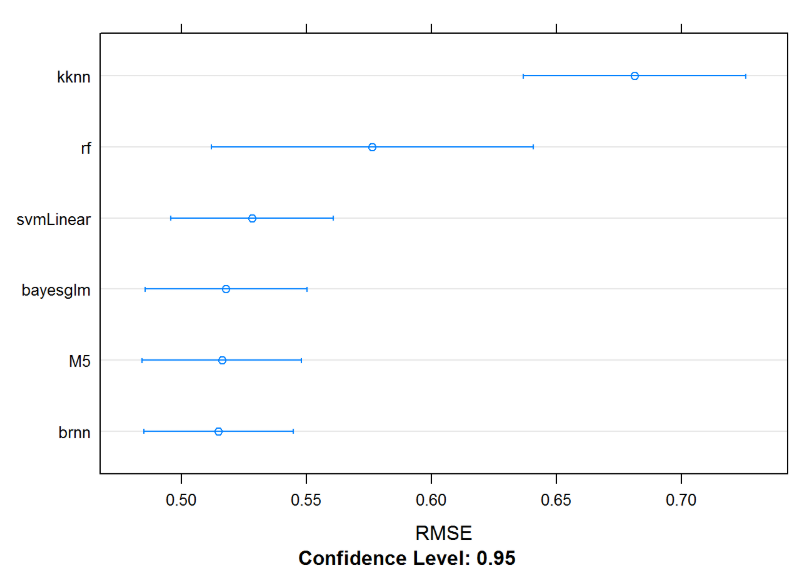
\includegraphics[width=0.6\textwidth]{recursos/ImagenesR/ComparacionModelos}

\end{figure*}
\FloatBarrier

Como se puede observar, las redes neuronales es el modelo que mejor precisión aportan utilizando los datos actuales. Este modelo es el que se usa para realizar la predicción de datos futuros.
\end{subappendices}



